\documentclass[a4paper]{article}

%--------------------------------------------------------------------------

\usepackage[a4paper, total={6in, 9in}]{geometry}
\usepackage{amsmath}
\usepackage{booktabs}
\usepackage{caption}
\usepackage{enumitem}
\usepackage{graphicx}
\usepackage{float}
\usepackage{inconsolata}
\usepackage{listings}
\usepackage{pstricks-add}
\usepackage{siunitx}
\usepackage[most]{tcolorbox}
\usepackage{tikz}
\usepackage{epstopdf} %converting to PDF
\usepackage{hyperref}
\usepackage{makecell}
\usepackage{siunitx}

\usetikzlibrary{shapes.geometric}

%------------------------------------------------------------
\graphicspath{{./fig/}}

%------------------------------------------------------------
\setlength{\parindent}{0in}

\lstdefinestyle{Python}{
	language        = Python,
	basicstyle      = \ttfamily,
	keywordstyle    = \color{blue},
	keywordstyle    = [2] \color{teal}, % just to check that it works
	stringstyle     = \color{green},
	commentstyle    = \color{red}\ttfamily
}

%------------------------------------------------------------
\newtcblisting[auto counter]{sexylisting}[2][]{sharp corners, 
    fonttitle=\bfseries, colframe=gray, listing only, 
    listing options={basicstyle=\ttfamily,language=Python}, 
    title=Listing \thetcbcounter: #2, #1}

%--------------------------------------------------------------------------

\begin{document}
\title{Udacity: Follow Me Report}
\author{Shane Reynolds}
\maketitle
\tableofcontents

\newpage

\section{Introduction}
Computer vision is a subset of robotic perception - it has been defined as the development of autonomous systems which can perform tasks achieved by human visual systems (Huang, 1996). This means the acquisition of digital image data from an optical camera, and some type of interpretation of the acquired image. A simple example of a task that is routinely performed by a human visual system, which is sought for computer vision systems, is answering the question: \textit{Is there a puppy in Figure 1?}, or \textit{Where is the puppy in Figure 1?}.
\begin{figure}[h]
\centering
\frame{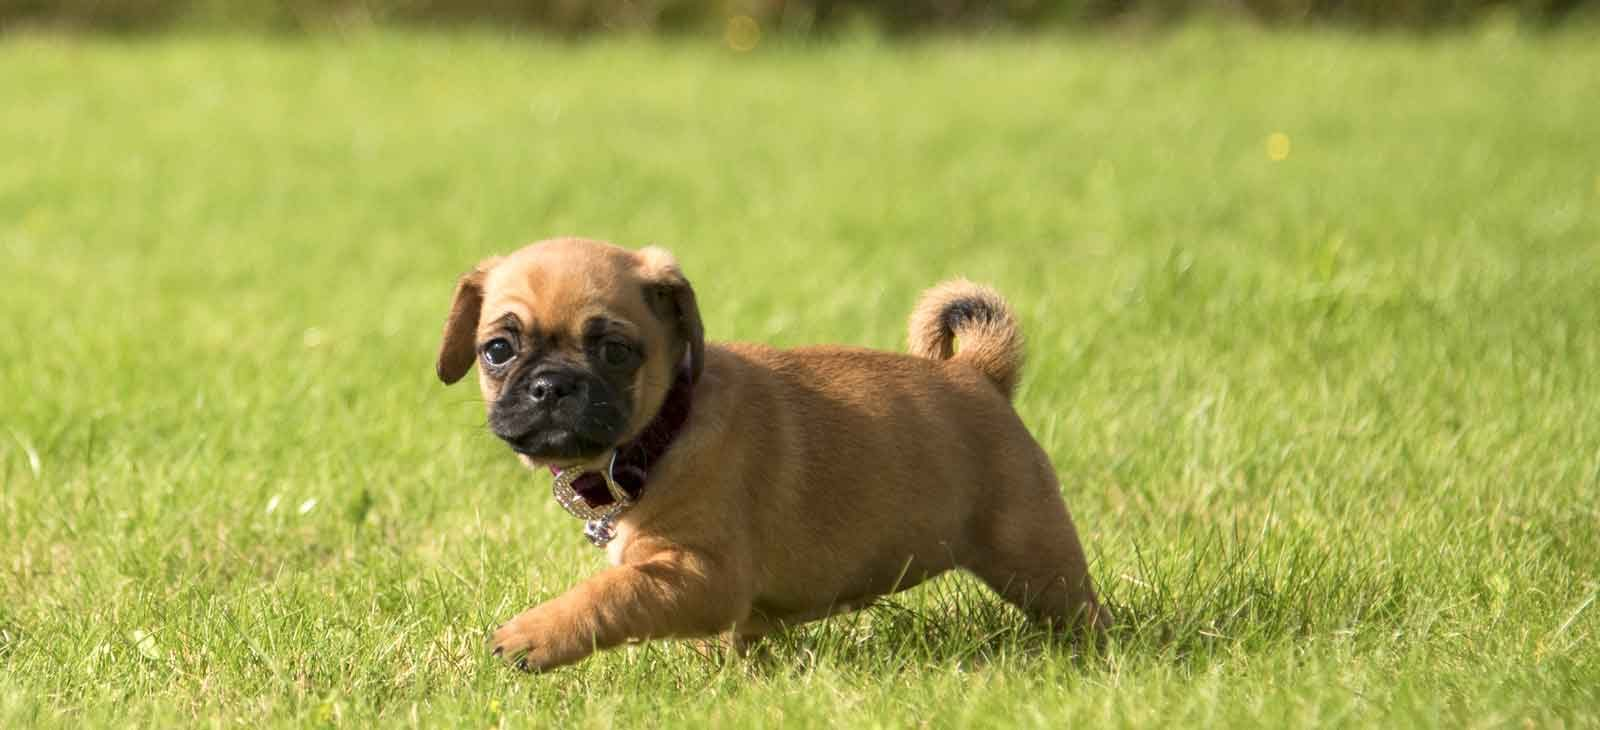
\includegraphics[scale=0.15]{puppy}}
\caption{Computer vision is interested in answering questions such as \textit{Is there a puppy in the image?} or \textit{Where is the puppy in the image?}}
\end{figure}

There are many sub-fields of computer vision such as scene reconstruction, event detection, video tracking, object recognition, 3D pose estimation, and motion estimation. This paper will focus on classification, using an approach called semantic segmentation. Shelhamer, Long and Darrell (2016) define semantic segmentation as a method of inference which is able to categorise fine image details. This is achieved by classifying each pixel in the image, and labelling it with the class of its enclosing object or region. A Fully Convolutional Neural Network (FCN) is proposed as the architecture to implement semantic segmentation. An FCN model was trained and implemented on a robotic agent.

\begin{figure}[h]
\begin{minipage}{0.45\textwidth}
\centering
\frame{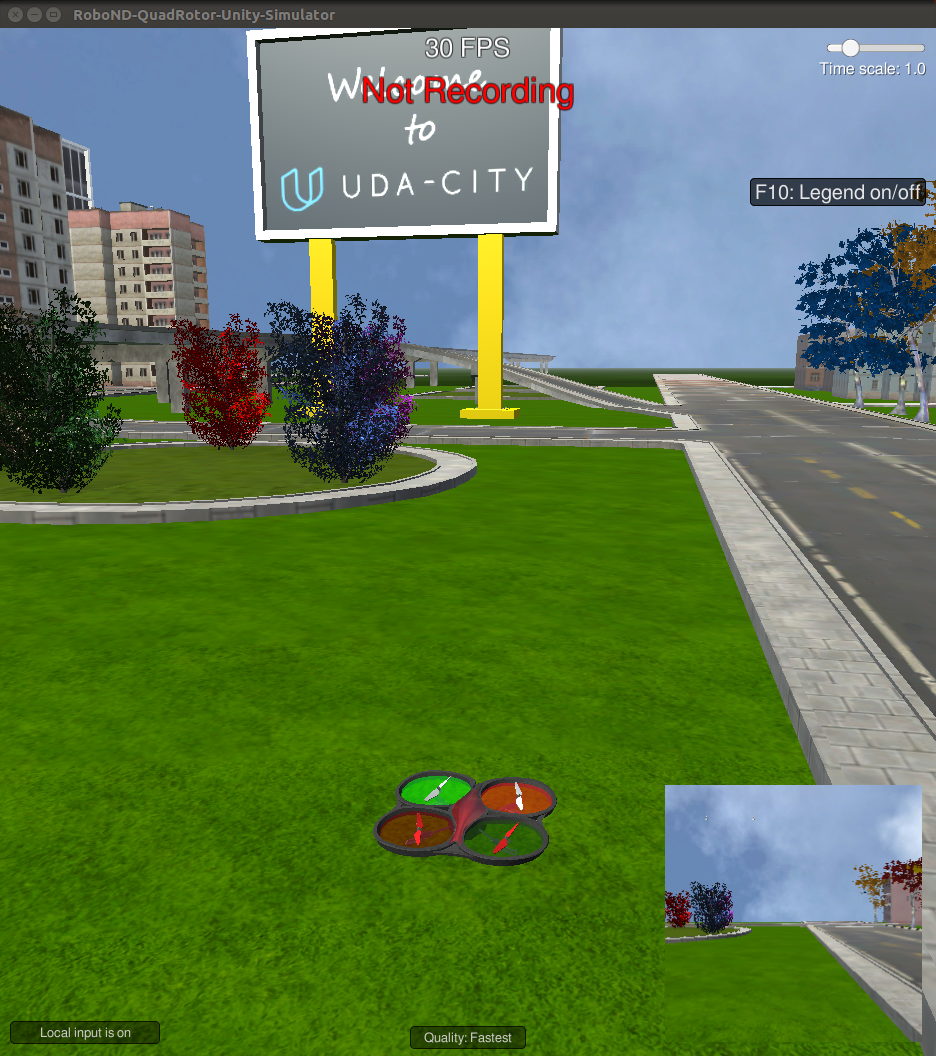
\includegraphics[height=6cm]{agent_image}}
\caption{The UAV agent in the simulated environment.}
\end{minipage}
\hspace{1cm}
\begin{minipage}{0.45\textwidth}
\centering
\frame{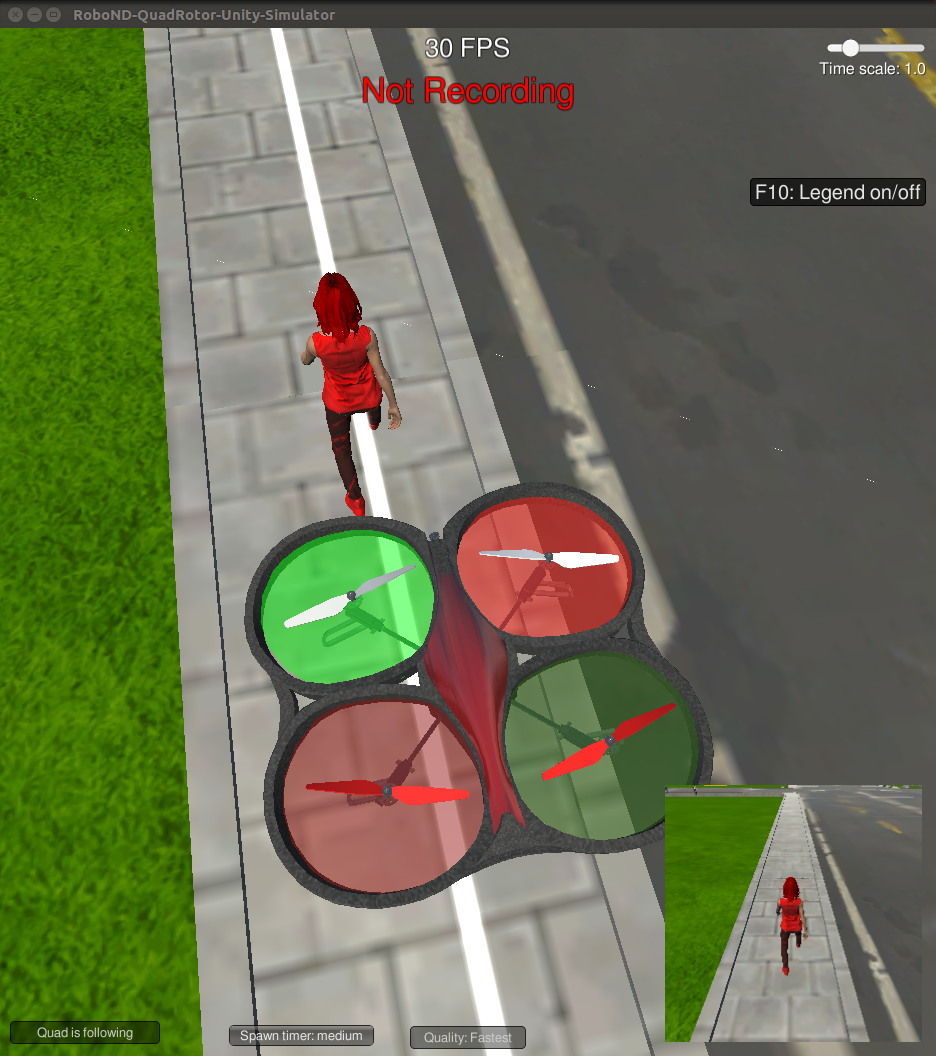
\includegraphics[height=6cm]{hero_image}}
\caption{The \textit{hero} can be seen coloured in red, with the UAV agent following her.}
\end{minipage}
\end{figure}

The agent was tasked with the identification (and subsequent tracking) of an individual, known as the \textit{hero}, in a 3D simulated environment built with Unity. The 3D simulated environment is a small city consisting of buildings, roads, elevated highways, and vegetation. The robotic agent is an unmanned aerial vehicle (UAV), as shown in Figure 2, which is fitted with a panning optical camera. The agent roams the simulation until it is able to locate the hero using the trained FCN, at which point the UAV will track the hero. The hero is a simulated person, as seen in Figure 3.

\section{Network Architecture}
FCNs are widely used for computer vision applications, and are a type of Artificial Neural Network (ANN). ANNs are computational models which, once trained on a dataset, can be used to make classification predictions, or  value estimations, based on a set of feature inputs that the model has been trained on. A typical fully connected feed-forward ANN consists of an input layer, one or more hidden layers, and an output layer, as shown in Figure 4. Hidden layers are made up of multiple nodes. The nodes themselves contain a non-linear activation function, such as a sigmoid or ReLU, and receive weighted input from the previous layers in the model. The inputs from the previous layer, and the non-linear activation of a node form a computational element called a neuron (also known as a perceptron) - these can be loosely thought of as decision making elements. An example of a neuron can seen in Figure 5.
\begin{figure}[h]
\begin{minipage}{0.45\textwidth}
\centering
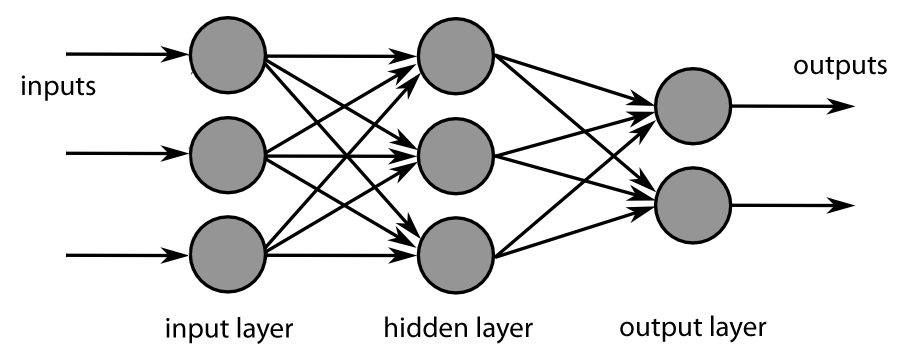
\includegraphics[scale=0.25]{feed_forward_neural_net}
\caption{A feed-forward artificial neural network consists of an input layer, which receives feature inputs, some hidden layers, and an output layer for classification.}
\end{minipage}
\hspace{1cm}
\begin{minipage}{0.45\textwidth}
\centering
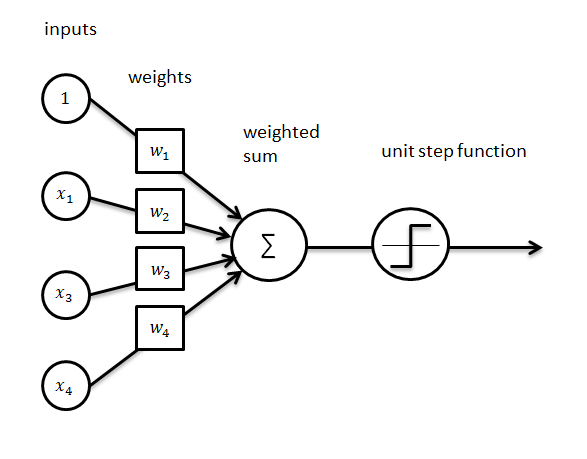
\includegraphics[scale=0.55]{perceptron}
\caption{The structure of a neuron (perceptron) includes weighted inputs from the previous layer, and a non-linear activation function.}
\end{minipage}
\end{figure}

Changing the weights in a neuron changes the neurons's contribution to the model, which in turn affects the overall model output. Weight changes occur during model training, which uses large volumes of labelled data to adjust the weights. Hidden layers are important because they allow highly non-linear models to be constructed, providing an approach for estimating complex phenomena which may be difficult to model with classical approaches, or computationally intractable. Generally, the more hidden layers, the more non-linear the model. Network architectures with multiple hidden layers have become so wide spread that the term Deep Neural Network (DNN) was coined to describe feed-forward ANNs which use two or more hidden layers. It must be noted that whilst increased non-linearity may allow us to model more complex phenomenon, making the ANN deeper does not guarantee increased model performance. This is mainly due to the fact that deeper models may over-fit the data during training, resulting in a failure to generalise on test and validation data sets.  

\begin{table}[h]
\centering
\caption{Reproduced from Ciresan, Meier, Gambardella, and Schmidhuber (2010) - DNN architectures of varying size for classifying the MNIST data set, and the associated performance of each network.} \footnotesize
\begin{tabular}{lS[table-format=3.2]S[table-format=3.2]S[table-format=3.2]S[table-format=3.2]}
\toprule
{\textbf{Architecture}} & {\textbf{Test Error}} & {\textbf{Best Test}} & {\textbf{Simulation}} & {\textbf{Weights}}\\
{\textbf{(number of neurons in each layer)}} & {\textbf{Best Validation [\%]}} & {\textbf{Error [\%]}} & {\textbf{Time [min]}} & {\textbf{[Millions]}}\\
\midrule
1000, 500, 10 & 0.49 & 0.44 & 23.4 & 1.34\\
1500, 1000, 500, 10 & 0.46 & 0.40 & 44.2 & 3.26\\
2000, 1500, 1000, 500, 10 & 0.41 & 0.39 & 66.7 & 6.69\\
2500, 2000, 1500, 1000, 500, 10 & 0.35 & 0.32 & 114.5 & 12.11\\
9 $\times$ 1000, 10 & 0.44 & 0.43 & 107.7 & 8.86\\
\bottomrule
\end{tabular}
\end{table}

Fully connected feed-forward DNNs have proven effective in computer vision classification problems, such as optical character recognition. One of the most widely cited examples of this is a feed-forward DNN performing classification on the MNIST dataset. The MNIST dataset contains handwritten digits, from 0 to 9, and is considered a benchmark for measuring neural net classification performance for the optical character recognition problem. Table 1, taken from paper by Ciresan, Meier, Gambardella, and Schmidhuber (2010), shows a table of feed-forward DNNs with varying numbers of hidden layers, and hidden layer depth.

\vspace{0.5cm}

\begin{minipage}{0.45\textwidth}
Notably, every model listed presents an error rate of less than 1\%. Generally, the deeper a network, the better the model's predictive performance, although this is not always the case as previously outlined. Figure 5, taken from the same paper, shows a small set of the misclassified images. Despite the misclassification it can be seen that, in most cases, the handwritten digit bears a high resemblance to the predicted value, and that the second prediction is generally correct. Remarkably, DNNs are not considered state of the art for image classification problems - even with simple tasks like MNIST classification. This is due to model inefficiencies that arise from image variation in the spatial domain.
\end{minipage}
\hspace{1cm}
\begin{minipage}{0.45\textwidth}
\centering
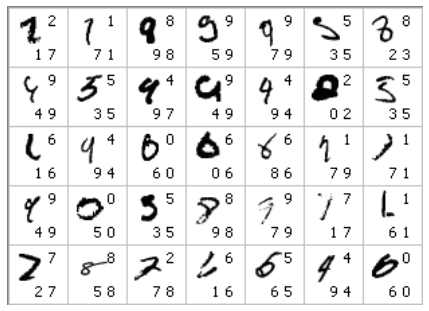
\includegraphics[height=3.5cm]{misclassification}
\captionof{figure}{Misclassified hand written digits by the top performing DNN from Ciresan, Meier, Gambardella, and Schmidhuber (2010). The digit in the top right hand corner of the box is the observation label, and the two digits in the bottom right hand corner are the predictions from the DNN model.}
\end{minipage}

\vspace{0.5cm}

The problem can be better understood by considering Figures 7 and 8. Figure 7 shows an image with a puppy on the left, and Figure shows an image with a puppy on the right. Suppose we create a simple model to classify whether an image has a puppy in it or not, and assume we train this model with lots of images like the one shown in Figure 7. If the trained model was then used to classify images like the one shown in Figure 8 it would perform poorly. This is because our model would have only learned to classify pixel features on the left side of the picture with puppies, which says nothing about identifying a puppy on the right hand side of an image. Put simply, there is no \textit{translational invariance} in the model.

\vspace{0.25cm}

\begin{figure}[h]
\begin{minipage}{0.45\textwidth}
\centering
\frame{
\includegraphics[height=4cm]{doggo_left}}
\caption{An image in which a puppy is located on the left hand side of the image.}
\end{minipage}
\hspace{1cm}
\begin{minipage}{0.45\textwidth}
\centering
\frame{
\includegraphics[height=4cm]{doggo_right}}
\caption{An image in which a puppy is located on the right hand side of the image.}
\end{minipage}
\end{figure}

\newpage

\subsection{Convolutional Neural Networks}
A Convolutional Neural Network (CNN) is a class of ANN, which has an underlying network structure which is better at learning shapes, edges, and colours meaning it is less reliant on the spatial location of a classification object in an image. Recall that vanilla feed-forward neural nets only have neuron connections from the previous layer, and there are no connections from neurons in the same layer - weights are not shared. In contrast, CNNs share neuron weights by using filters which are convolved over an input image. Consider a raw input image of say 32 $\times$ 32 pixels, with a depth of 3 colour channels, as shown in Figure 9.
\begin{figure}[h]
\begin{minipage}{0.45\textwidth}
\centering
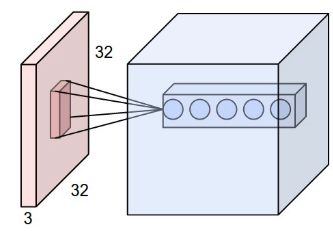
\includegraphics[scale=0.4]{CNN}
\caption{The raw image input is 32 $\times$ 32, with a 3-channel depth (R,G,B). The filter is a 3 $\times$ 3 patch with the same depth as the input. The filter is convolved over the image using some stride - each convolution creates a single element output which forms part of the 2D activation map (i.e. the output). There are $K$ filters convolved over the image, a parameter chosen as part of the architecture, and the output volume represents the stacked 2D activation maps.}
\vspace{0.5cm}
\end{minipage}
\hspace{1cm}
\begin{minipage}{0.45\textwidth}
\centering
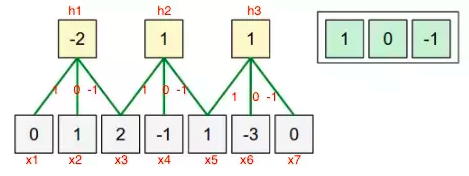
\includegraphics[scale=0.43]{CNN_example}
\caption{An simple example of weight sharing that takes place in a CNN. The white 1D array represents the input image, and the blue 1D array represents the filter. The filter (blue) is convolved across the input (white) using a stride of 2. The convolved output, which represents the activation map, can be seen in yellow. This architecture allows for the sharing of the weights in the model.}
\end{minipage}
\end{figure}

The convolving filter, which contains the model weights, is the small patch which is incident on the raw input image surface. The image section in contact with the filter is called the receptive field - this changes as the filter convolves an image. Filter width and height are parameters chosen as part of the network architecture, and filter depth is identical to the input image depth. The filter is moved around the image according to the number of pixels in each stride. After each movement, the filter weights are multiplied by the receptive field and added together - this makes up a single entry in the 2D activation map which forms part of the output volume. The width and height of the output volume are dependent on the stride, and the type of padding used during the convolution. Finally, the output depth is dependent on the number of filters specified in the network architecture - typically this parameter is denoted as $K$. The output volume is simply the stacked 2D activation maps from each filter. It is the convolutional process, whereby the filter weights are used over an entire image, that provide the weight sharing seen in CNNs. Figure 10 provides a simple example of how this works. In this example, the filter is a 1D array (shown in blue), and the input image is also a 1D array (shown in white). The filter (blue) is convolved over the input image (white) with a stride of 2. The filter weights are multiplied with the image values, and added together to form the output volume - a 1D array (shown in yellow).\\

CNNs provide superior performance over DNNs in the image classification domain. This was demonstrated on the MNIST dataset by LeCun (XXXX) with his LeNet (pictured in Figure 11), and again by Krizhevsky (XXXX) on the ImageNet dataset with AlexNet (shown in Figure 12). Whilst CNNs can achieve noteworthy performance in the task of image classification, there is a notable performance loss when they are re-tasked with pixel by pixel classification known as semantic segmentation. This is due to the fact that fully connected layers (the network classifiers) don't preserve spatial information.
\begin{figure}[h]
\centering
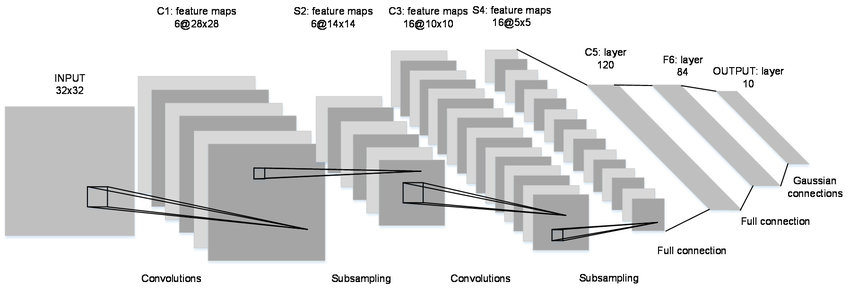
\includegraphics[scale=0.45]{lenet5}
\caption{text}
\end{figure}

\begin{figure}[h]
\centering
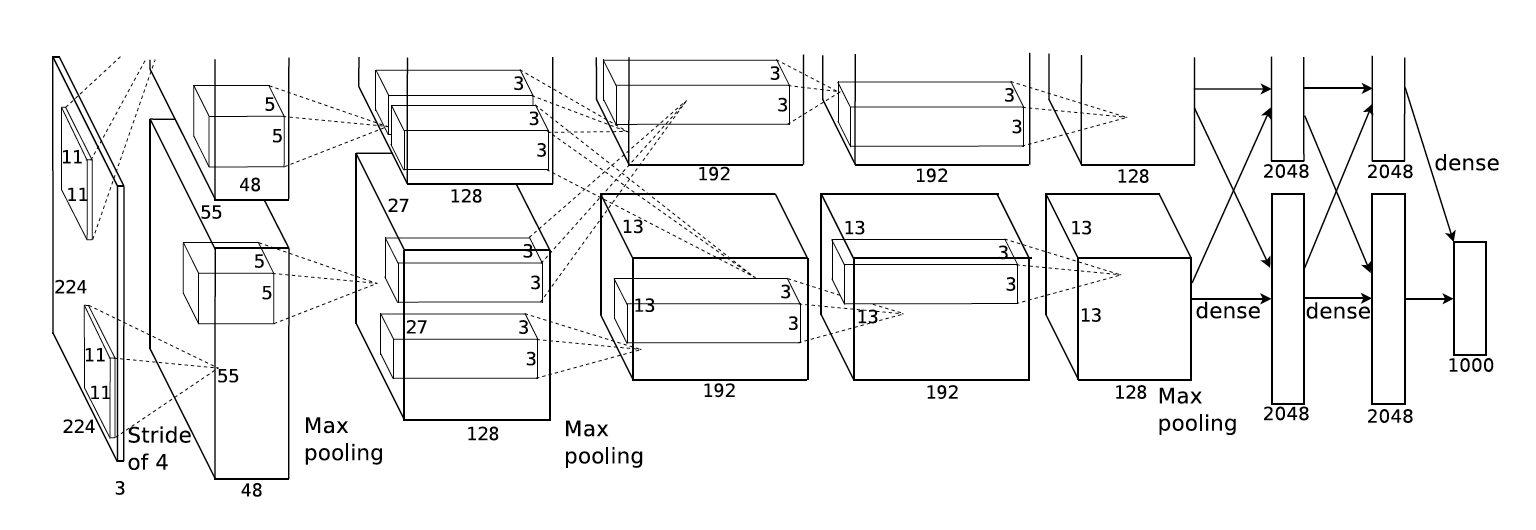
\includegraphics[scale=0.25]{alexnet}
\caption{text}
\end{figure}

\subsection{Fully Convolutional Neural Networks}
FCNs preserve spatial information, and represent a state-of-the-art approach to semantic segmentation. Structurally, they can be thought of as two distinct parts: encoders and decoders. This is shown in Figure 13. The encoder is comprised of several convolutional layers, which are typically arranged to progressively concentrate the spatial domain, and increase the number of channels in the image. These different layers of spatial compression are useful for training the model on different image resolutions. The decoder, in contrast, upsamples encoder compressions, restoring the spatial information to the output - typically the final layer restores the output to the initial input image dimensions, before being passed to a convolutional layer with a softmax activation function.
\begin{figure}[h]
\centering
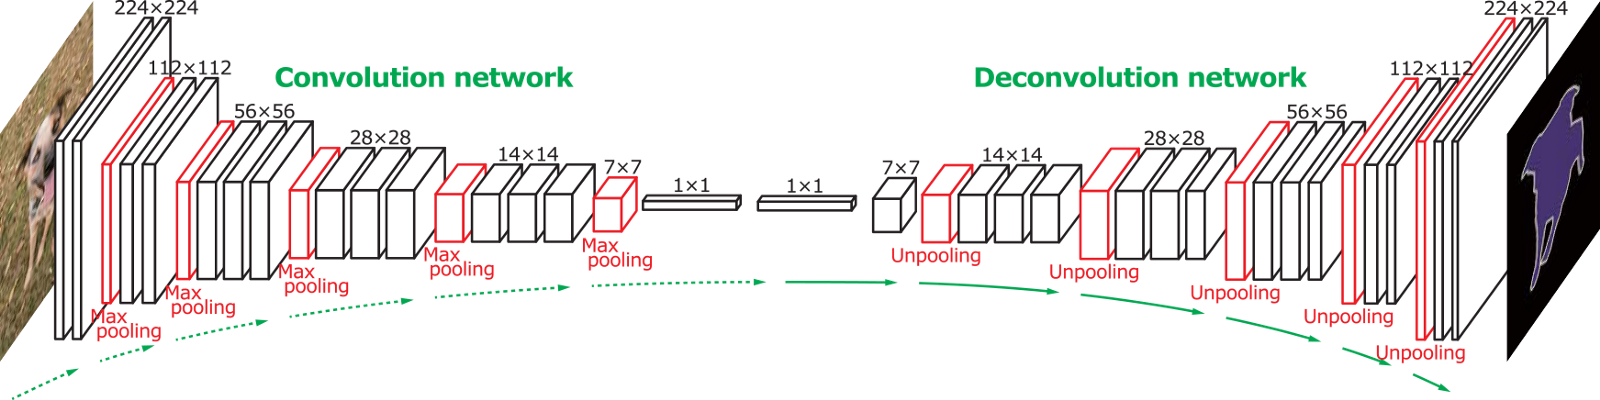
\includegraphics[scale=0.25]{FCN}
\caption{text}
\end{figure}

FCNs are often built with a 1 $\times$ 1 convolution bridging the gap between the encoder and decoder. A 1 $\times$ 1 convolution The reasons cited for using this architecture:
\begin{enumerate}
\item \textbf{Computational efficiency}:
\item \textbf{Increase network depth without incurring spatial deformation}: 
\end{enumerate}



\subsection{Proposed Architectures \& Implementation}
The 
\subsubsection{Model 1: Deep Model with 1 $\times$ 1 Convolution}
\subsubsection{Model 2: Shallow Model with 1 $\times$ 1 Convolution}
\subsubsection{Model 3: Shallow Model - No 1 $\times$ 1 Convolution}

\section{Network Training}
The initial data set provided with the problem was comprised of XXXX images. There are three rough categories that the images can be placed in:

%Talk about the pre-processing of the data set (what does this do?)

%Talk about the 

\subsection{Epochs}
Talk about epochs contributing to more data being passed through the model - the more epochs the better - post graphic

\subsection{Learning Rate}
Talk about the learning rate being critical to 

\subsection{Batch Size}

\section{Performance \& Model Generalisation}

\section{Future Enhancements}
% Collecting addtional datasets and filtering them to only include images of the hero - note that we want data that does not include the 
\end{document}